\section{Background and Related Works}
\label{sec:background}

We introduce %OIDC \cite{OpenIDConnect}, to describe
typical SSO login flows and discuss existing privacy-preserving solutions and other related works.

\subsection{OpenID Connect and SSO Services}
\label{subsec:OIDC}
%OIDC is one of the most popular SSO protocols.
OIDC supports three login flows: implicit flow, authorization code flow, and hybrid flow (a mix of the other two).
These flows differ in the steps for requesting and receiving identity tokens but have common security requirements for identity tokens.
We present our designs in the implicit flow and discuss the support for the authorization code flow in Section \ref{sec:discussion}.

In an OIDC system, users and RPs register at an IdP with their identities
and other information such as user credentials %(e.g., passwords)
and RP endpoints. %(i.e., the URLs to receive tokens).
As shown in Figure \ref{fig:OpenID}, when a user initiates a login request to an RP, the RP constructs an identity-token request with its own identity and the scope of the requested user attributes.
This request is redirected to a trusted IdP.
Once the IdP verifies the user's identity, it issues an identity token that encloses the identities (or pseudo-identities) of the user and the visited RP, the requested user attributes, a validity period, etc. The user then forwards the identity token to the RP's endpoint. The RP verifies the token and allows the holder to login as the enclosed (pseudo-)identity.
The user's operations, including request redirection, authorization, and token forwarding, are carried out through user agents, such as a browser for web applications.

\begin{figure}[t]
  \centering
  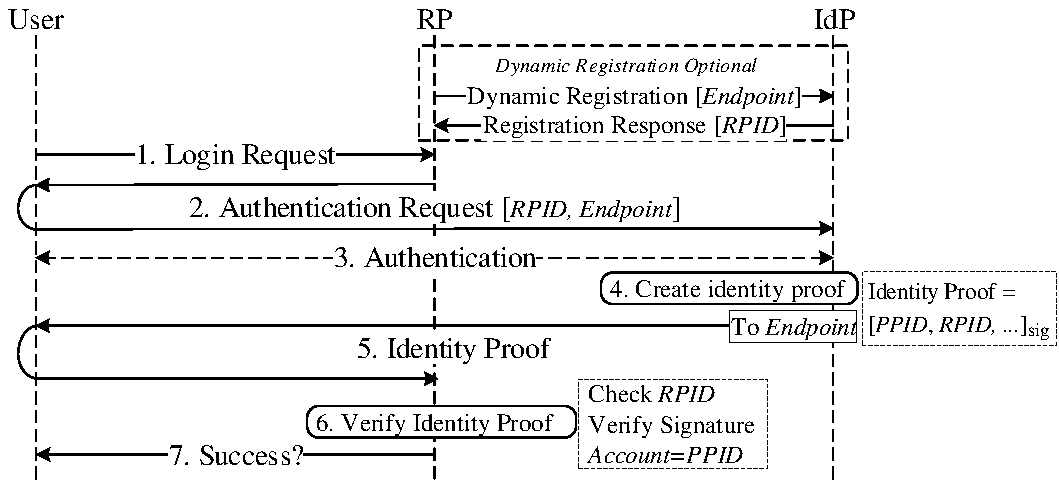
\includegraphics[width=0.98\linewidth]{fig/OIDC1.pdf}
  \caption{The implicit SSO login flow of OIDC}
  \label{fig:OpenID}
\end{figure}

\begin{table*}[tb]
\footnotesize
    \caption{Privacy-Preserving Solutions of SSO and Identity Federation}
    \centering
    \begin{tabular}{|c|c|c|c|c|c|c|}
  \hline
  \multirow{3}*{\textbf{~~Solution~~}} &
  \multicolumn{3}{c|}{\textbf{SSO Features} - supported $\CIRCLE$, unsupported $\Circle$, or partially $\LEFTcircle$} & \multicolumn{3}{c|}{\textbf{Privacy Threats} - prevented $\CIRCLE$ or not $\Circle$} \\ \cline{2-7}
  & User Identification & User Authentication & IdP-confirmed Selective  & IdP-based & RP-based & IdP-RP \\
  & at each RP & to only the IdP &  Attribute Provision & Login Tracing & Identity Linkage & Collusion \\\hline\hline
  OIDC w/ PPID \cite{NIST2017draft} & $\CIRCLE$ & $\CIRCLE$ & $\CIRCLE$ & $\Circle$ & $\CIRCLE$ & - \\ \hline
  BrowserID \cite{BrowserID} & $\CIRCLE$ & $\CIRCLE$$^1$ & $\Circle$ & $\CIRCLE$ & $\Circle$ & - \\ \hline
  SPRESSO \cite{SPRESSO} & $\CIRCLE$ & $\CIRCLE$ & $\LEFTcircle$$^2$ & $\CIRCLE$ & $\Circle$ & - \\ \hline \hline
  PRIMA \cite{prima} & $\CIRCLE$ & $\Circle$ & $\CIRCLE$ & $\CIRCLE$ & $\Circle$ & - \\ \hline
  PseudoID \cite{PseudoID} & $\CIRCLE$ & $\Circle$ & $\LEFTcircle$$^3$ & $\CIRCLE$ & $\CIRCLE$ & $\CIRCLE$ \\ \hline
  Opaak \cite{Opaak} & $\LEFTcircle$$^4$ & $\Circle$ & $\Circle$ & $\CIRCLE$ & $\CIRCLE$ & $\CIRCLE$ \\ \hline
  U-Prove \cite{uprov} & $\CIRCLE$ & $\Circle$ & $\LEFTcircle$$^5$ & $\CIRCLE$ & $\CIRCLE$ & $\CIRCLE$ \\ \hline
  UnlimitID \cite{UnlimitID} & $\CIRCLE$ & $\Circle$ & $\CIRCLE$ & $\CIRCLE$ & $\CIRCLE$ & $\CIRCLE$ \\ \hline
  EL PASSO \cite{ELPASSO} & $\CIRCLE$ & $\Circle$ & $\CIRCLE$ & $\CIRCLE$ & $\CIRCLE$ & $\CIRCLE$ \\ \hline
  Fabric Idemix \cite{hyperledge-idemix} & $\LEFTcircle$$^6$ & $\Circle$ & $\CIRCLE$ & $\CIRCLE$ & $\CIRCLE$ & $\CIRCLE$ \\ \hline\hline
 % PrivacyPass \cite{privacypass,trusttoken} & $\Circle$ & $\Circle$ & $\Circle$ & $\CIRCLE$ & $\CIRCLE$ & $\Circle$ \\ \hline
  UPPRESSO & $\CIRCLE$ & $\CIRCLE$ & $\CIRCLE$ & $\CIRCLE$ & $\CIRCLE$ & $\Circle$ \\ \hline
\end{tabular}
    \label{tbl:comparison-protocol}
\flushleft
{\footnotesize
1. A BrowserID user generates an \emph{ephemeral} private key to sign the ``subsidiary'' token,
 which is also verified by the RP.\\
2. SPRESSO can be extended to provide user attributes in the tokens, while the prototype does not implement this feature.\\
3. Blindly-signed user attributes can be selectively provided using zero-knowledge proofs but not implemented in the prototype.\\
4. Opaak supports two exclusive pseudonym options: (\emph{a}) linkable within an RP but unlinkable across multiple RPs and (\emph{b}) unlinkable for any pair of actions.\\
5. The U-Prove token may contain attributes that are \emph{invisible} to the IdP in addition to the ones confirmed by the IdP. \\
6. In the original design of Idemix \cite{idemix}, every user logs in to an RP with a unique account, but Fabric Idemix implements completely-anonymous services.
}
\end{table*}

The following three features are desired in SSO services and supported by popular SSO systems \cite{NIST2017draft, OpenIDConnect,rfc6749, SAML, SAMLIdentifier}.

\noindent \textbf{User identification at an RP.}
An RP recognizes each user by a \emph{unique} identity or account at the RP to provide customized services across multiple different login instances.
Such \emph{non-anonymous} services are more desirable in various applications than anonymous SSO.

\noindent\textbf{User authentication to {\em only} an IdP.}
%A widely-adopted SSO protocol  usually does not include authentication steps.
In widely-used SSO protocols \cite{OpenIDConnect, rfc6749, SAML}, RPs only verify the identity tokens issued by an IdP, and the authentication between a user and the IdP is typically conducted \emph{independently} of the steps that deal with identity tokens. This approach offers several advantages. First, the IdP authenticates users using any appropriate means such as passwords, one-time passwords, or multi-factor authentication.
%It eliminates the authentication steps between users and an RP,
Meanwhile, a user only maintains his credential at the IdP; and if it is lost or leaked, the user only needs to renew it at the IdP.
However, if a user proves a \emph{non-ephemeral secret} to RPs that is valid across multiple login instances, he will have to notify each RP in the event of loss or leakage, or additional revocation checking will be needed \cite{ELPASSO, UnlimitID}.

%. %(or even the user logins from another computer).

\noindent\textbf{Selective IdP-confirmed attribute provision.}
An IdP usually includes user attributes in identity tokens \cite{OpenIDConnect,rfc6749} with user (pseudo-)identities.
A user maintains these attributes at the trusted IdP,
%    for example,
%        when Facebook provides social networking services,
%         it also issues identity tokens enclosing user identities and various attributes.
which obtains the user's authorization before including attributes or provides only pre-selected attributes.
%So no distinctive attributes such as telephone number and Email address are enclosed in the identity tokens of privacy-preserving SSO systems.

\subsection{Privacy-Preserving SSO and Identity Federation}
\label{subsec-solutions}

SSO protocols \cite{OpenIDConnect,rfc6749, SAML, SAMLIdentifier} allow users to login to an RP
 \emph{without maintaining an account at the RP or holding a permanent secret to be verified by the RP}.
Privacy-preserving SSO is expected to offer the desired features as above,
    while addressing different types of privacy threats.
On the other hand,
  identity federation enables a user registered with a trusted IdP to be accepted by other parties, potentially with different accounts,
   but \emph{additional user operations for the authentication steps between the user and RPs} are involved while more privacy threats are prevented.\footnote{Although the term ``single sign-on (SSO)'' was used in several schemes \cite{PseudoID, Opaak, ELPASSO, WangWS13, HanCSTW18, HanCSTWW20},
    they are very different from widely-used SSO protocols,
    where a user needs to maintain the accounts at different RPs and/or hold a permanent secret verified by the RPs.
So in this paper we call them \emph{identity federation} to emphasize this difference.}
However, as shown in
    Table \ref{tbl:comparison-protocol}, none of the existing solutions satisfies all the requirements.



\noindent\textbf{Privacy-preserving SSO.} %While supporting these features,
Existing privacy-preserving SSO approaches \cite{BrowserID, SPRESSO, NIST2017draft} prevent either IdP-based login tracing or RP-based identity linkage, but not both. %and UPPRESSO prevents both of them.
Pairwise pseudonymous identifiers (PPIDs) are specified \cite{OpenIDConnect, SAMLIdentifier} and recommended \cite{NIST2017draft}
for protecting user privacy against curious RPs.
An IdP creates a unique PPID for a user to login to some RP and encloses it in identity tokens,
 so colluding RPs cannot link the user's identities.
It cannot prevent IdP-based login tracing because the IdP needs the RP's identity to assign PPIDs.

Other privacy-preserving SSO schemes prevent IdP-based login tracing but leave users vulnerable to RP-based identity linkage, due to the unique user identities used in identity tokens.
For example, in BrowserID \cite{BrowserID} %(formerly known as Firefox Accounts \cite{FirefoxAccount} and Mozilla Persona \cite{persona}),
the IdP %(called the primary identity authority in BrowserID)
issues a ``user certificate'' token that binds a user identity to an ephemeral public key. The user then signs a subsidiary ``identity assertion'' token that includes the target RP's identity and sends both tokens to the RP.
In SPRESSO \cite{SPRESSO} the RP creates a one-time pseudo-identity in each login instance, which is included in identity tokens with the user's unique identity.

%However, colluding RPs can link a user using the unique identity in the tokens or credentials.

\noindent\textbf{Privacy-preserving identity federation.} In PRIMA \cite{prima} the IdP signs a credential
%\footnote{For the message signed by the IdP works with a user secret verified by an RP,
%    it is usually called a credential  in identity federation instead of token.}
that binds user attributes and a verification key. Using the signing key, the user selectively provides attributes to the RPs. %\cite{Oblivion}.
This verification key works as the user's identity but exposes her to RP-based identity linkage.

To protect user privacy against more threats, PseudoID \cite{PseudoID} introduces a service in addition to the IdP,
 to \emph{blindly} sign %\cite{blind-sign}
an access token that binds a pseudonym and a user secret. The user unblinds this token and uses the secret to login to an RP. Approaches based on anonymous credentials \cite{anon-credential-2001, idemix, anon-credential} have been proposed to implement privacy-preserving identity federation \cite{hyperledge-idemix, Opaak, uprov, UnlimitID, ELPASSO}. For instance, the IdP signs anonymous credentials in Opaak \cite{Opaak}, UnlimitID \cite{UnlimitID}, EL PASSO \cite{ELPASSO}, and U-Prove \cite{uprov,uprove-conference}, and binds them with non-ephemeral user secrets. %, with which users can authenticate to an RP.
The users prove ownership of the anonymous credentials using the secrets
 and disclose IdP-confirmed selective attributes in the credentials in most approaches except Opaak.
Similarly, Hyperledger Fabric \cite{hyperledge-idemix} integrates the Idemix anonymous credentials \cite{idemix} for completely-unlinkable pseudonyms and IdP-confirmed attribute disclosure.

These approaches prevent both IdP-based tracing and RP-based identity linkage,
 for (\emph{a}) the RP's identity is not included in the anonymous credentials and
  (\emph{b}) the user selects different pseudonyms when visiting different RPs.
Furthermore, they protect user privacy against collusive attacks by the IdP and RPs, as \emph{user-managed} pseudonyms cannot be linked through anonymous credentials \cite{anon-credential-2001, idemix, anon-credential} even when the ownership of these credentials is proved to RPs using one secret.
%This approach can prevent both privacy threats since (\emph{a}) the RP's identity is not included in the tokens and (\emph{b}) the user can select different pseudonyms when visiting different RPs. Furthermore, PseudoID prevents collusive attacks by the IdP and RPs because they cannot link two blindly-signed tokens.
However, this privacy protection results in additional user operations in identity federation compared with widely-used SSO.
Users are required to maintain not only the authentication credentials for the IdP but also the long-term secrets that are verified by RPs.
For example, EL PASSO \cite{ELPASSO} requires users to store the secrets securely on their devices and coordinate the credential revocation process \cite{ELPASSO, UnlimitID}.
Besides, the users need to manage their accounts at different RPs locally. This actually involves authentication steps between the user and RPs, which is usually referred to as asynchronous authentication \cite{ELPASSO}.

%EL PASSO \cite{ELPASSO} is an identity federation solution that uses anonymous credentials to protect user privacy. After a user is authenticated, the IdP signs an anonymous credential \cite{anon-credential} binding a secret, which is securely kept on the user's device. When logging in to an RP, the user proves ownership of the credential using the secret and discloses selective attributes in the credential. Although one credential is proved to multiple RPs, the use of \emph{user-managed pseudonyms} and \emph{anonymous credentials} prevents RPs, which may collude with the IdP, from linking a user across different RPs.

%Similarly, UnlimitID \cite{UnlimitID} uses anonymous credentials \cite{anon-credential} to prevent collusive attacks by the IdP and RPs, and NEXTLEAP \cite{nextleap} builds on top of UnlimitID to provide anonymous messaging.

%Anonymous credentials \cite{anon-credential-2001,anon-credential} have been proposed for flexible uses.


\noindent\textbf{Anonymous identity federation.} Such schemes protect user privacy completely:
  a trusted IdP issues credentials for a user to access RPs with pseudonyms which are unlinkable for any pair of access actions.
Anonymous identity federation systems have been formalized \cite{WangWS13}
    and solutions \cite{WangWS13, HanCSTW18, HanCSTWW20} are proposed using different cryptographic primitives such as group signature and zero-knowledge proof.
Sometimes, special features (e.g., designated verifier \cite{HanCSTW18} and proxy re-verification \cite{HanCSTWW20}) are also designed.
%and proposed for different applications such as GSM communications \cite{ElmuftiWRR08},
% However, they cannot support user identification at the RPs.
These completely-anonymous authentication services only work for some special scenarios,
 but do not support user identification at an RP,
    which is commonly desired in most applications.
